
\subsection{Introduction}

Water tank edges in MR images contains the z-axis distortion information. Combining with water tank edges in 
CT images, z-axis correction parameters could estimated using least square fitting method. \\
Due to the similarity in physical location of the interested data points, algorithm used in water tank edge
extraction from CT images is a good candidate. However, there are some issue preventing that algorithm to be
applied directly on water tank edge extraction from MR images.

\begin{enumerate}
\item There are much more considerable noises in MR images than in CT images. Due to the length of the phantom 
  is slightly longer than the internal length of the headcoil, one water tank is slightly outside of the
  headcoil. This will results a much noise region on the water tank appear in lower region of MR images, as
  shown in figure ~\ref{fig:mri_noise_sample}.
\item Unlike CT images, the surfaces in MR images are curved. So we cannot use the same line fitting method
  we used in CT images water tank edges extraction.
\item Unlike CT images, we need as much data points as possible on each surface. Especially those ones on the
  edge. 
\end{enumerate}

\begin{figure}[htb]
  \hfill
  \begin{minipage}[b]{3in}
    \centering
    \centerline{\mbox{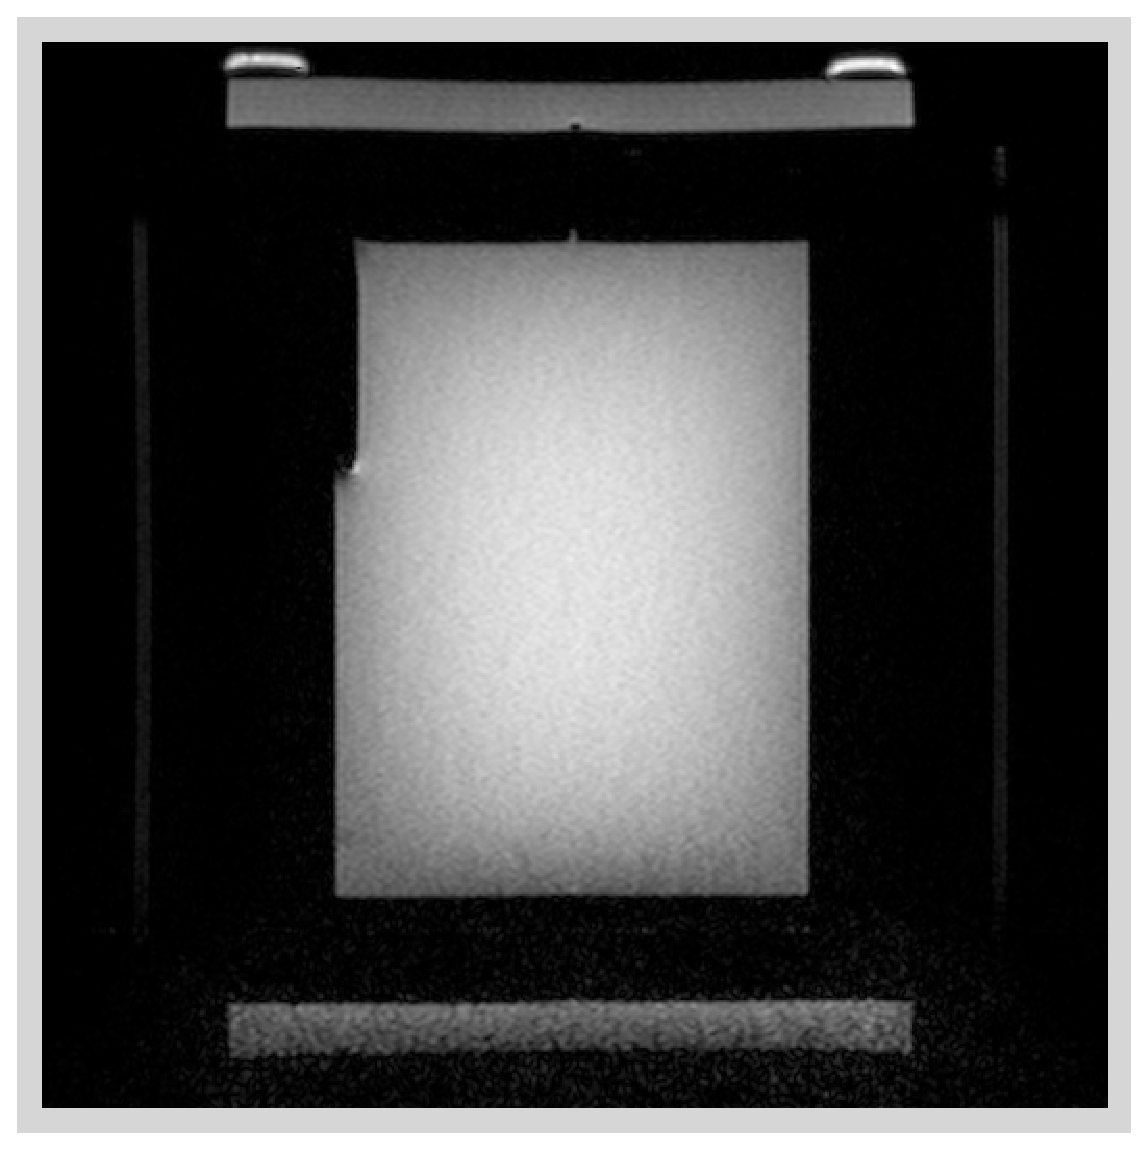
\includegraphics[width=3in]{data_extraction/images/MRI/sample_mri_phantom.eps}}}
  \end{minipage}
  \hfill
  \caption{Noisy MR images, especially the lower tank}
  \label{fig:mri_noise_sample}
\end{figure}

\subsection{Algorithm}

The algorithm used in water tank extraction in MR images is a modification of water tank extraction in CT
images, it can be described as follows:

\begin{enumerate}
  \item Find left and right boundaries. The algorithm of finding left and right boundary is the same as 
    as water tank edges extraction in CT images, except we only need to find the boundaries for top tank's
    lower surface. This is because before final MRI scan, the phantom is already aligned, MR tubes should 
    be quite parallel to the z-axis, and all four surfaces left and right boundary should be extremely close.
    In fact, top tank's lower surface's left and right boundary should be wider than other surfaces. This tight
    bound is sufficient for rest of the algorithm to work well.
  \item For each surface, instead of using canny algorithm to find initial raw edge, algorithm will iterate 
    from left boundary to right boundary to analyze the histogram of each column, and pick the maximum peaks
    with the highest value as a edge point. As shown in figure ~\ref{fig:mri_edge_point_histograms}.
    \begin{figure}[htb]
      \begin{center}
        \begin{minipage}[b]{3in}
          \centering
          \centerline{\mbox{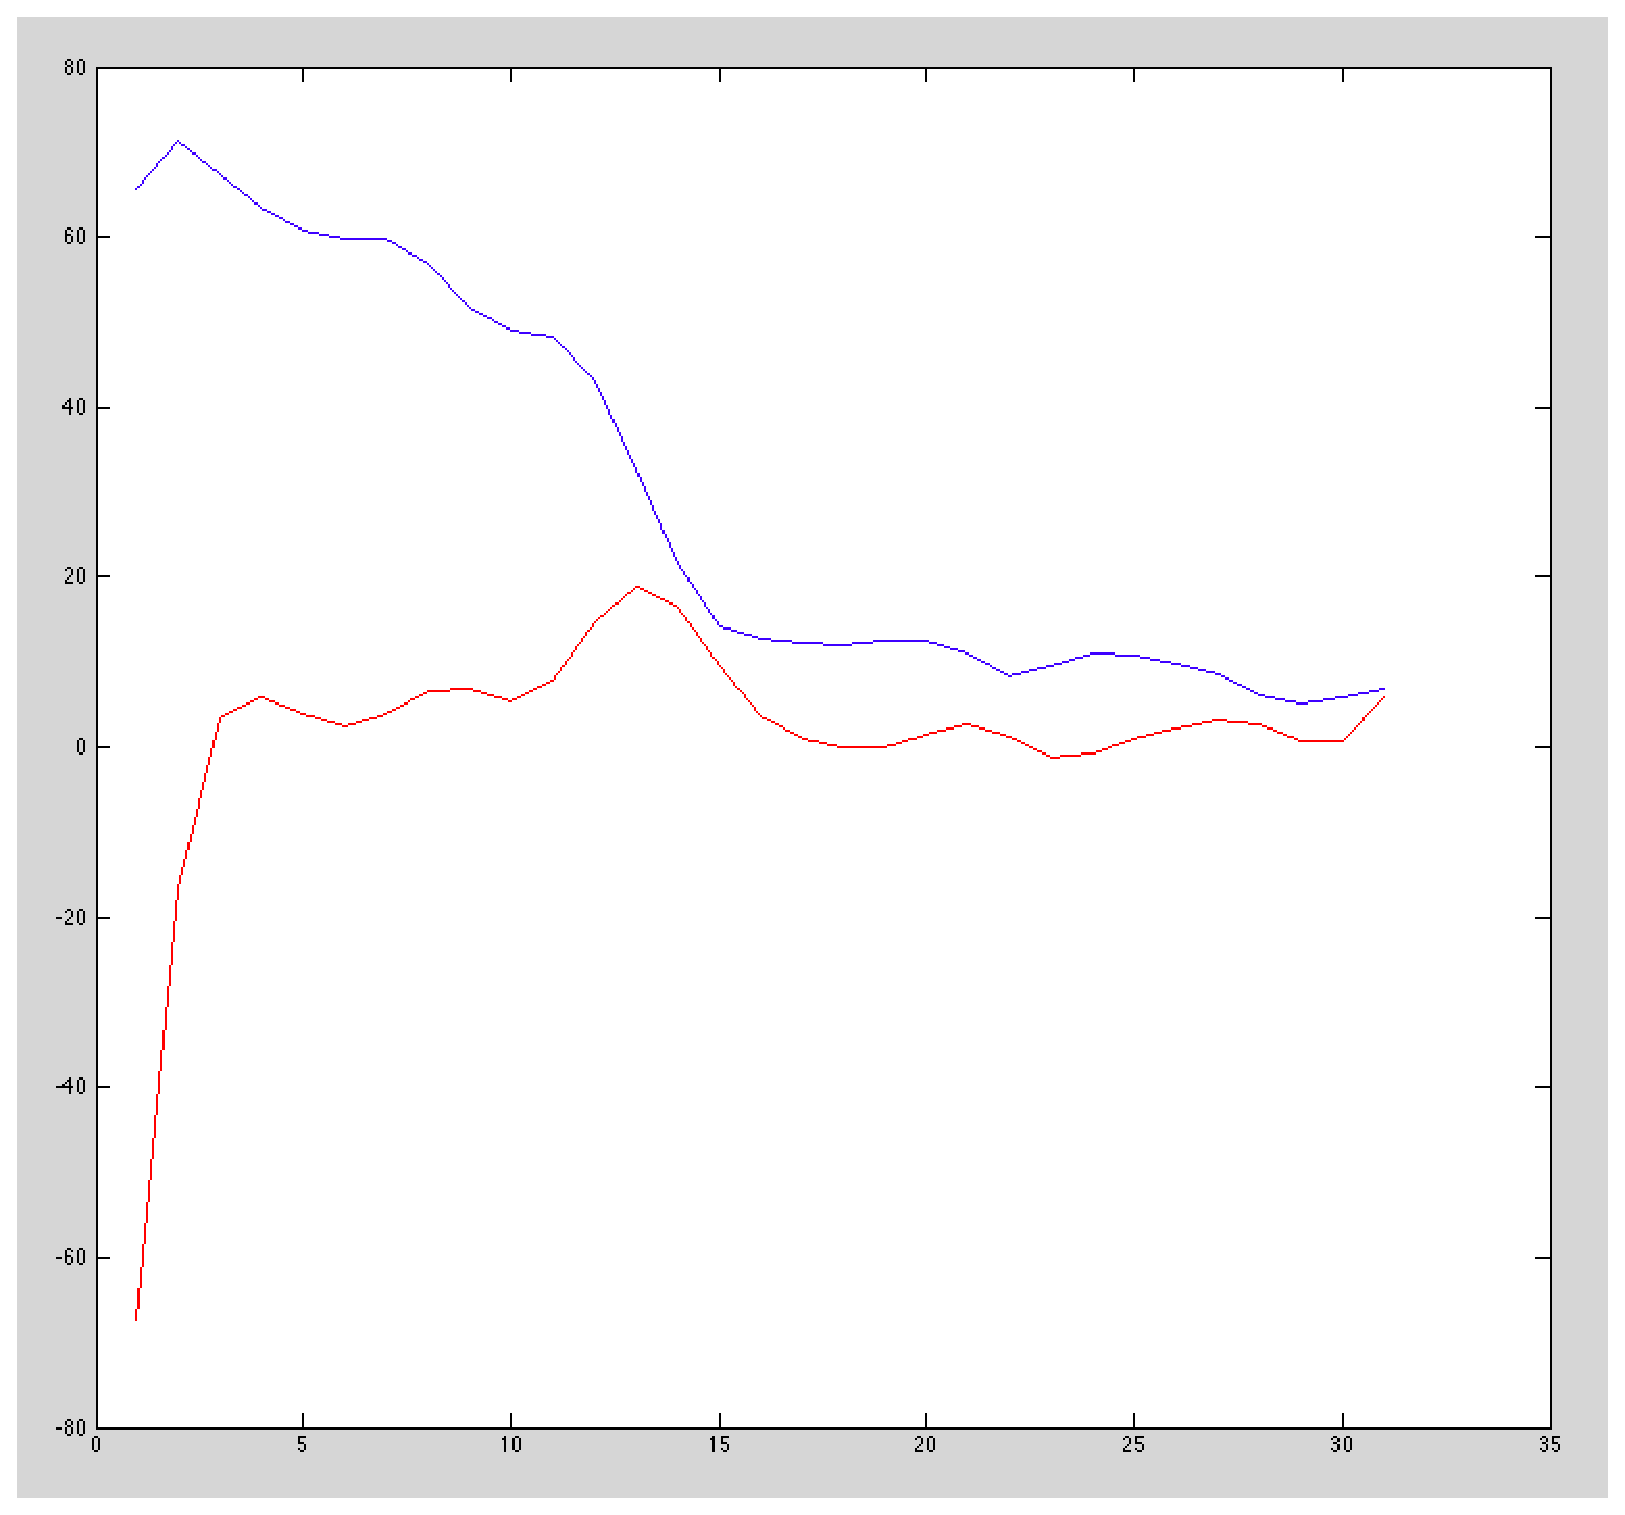
\includegraphics[width=3in]{data_extraction/images/MRI/find_edge_point.eps}}}
        \end{minipage}
      \end{center}
      \caption{Histogram for finding edge points}
      \label{fig:mri_edge_point_histograms}
    \end{figure}
  \item The resulting edge from previous step is very noisy. The following steps will be use to remove the
    noises. 
    \begin{enumerate}
      \item Remove disjointed short edges.
      \item By analyzing the gradient histogram, remove large disjointed edges.
      \item By analyzing the gradient histogram, remove short bumps in noisy edge.
      \item By analyzing the gradient histogram, remove all the sharp peaks. 
    \end{enumerate}
    The algorithm used to parse the gradient histogram is described in figure ~\ref{fig:histogram_state_machine}. Edge result after each step are shown in figure ~\ref{fig:mri_edge_results}.
\end{enumerate}

\begin{figure}[htb]
  \hfill
  \begin{minipage}[b]{5in}
    \centering
    \centerline{\mbox{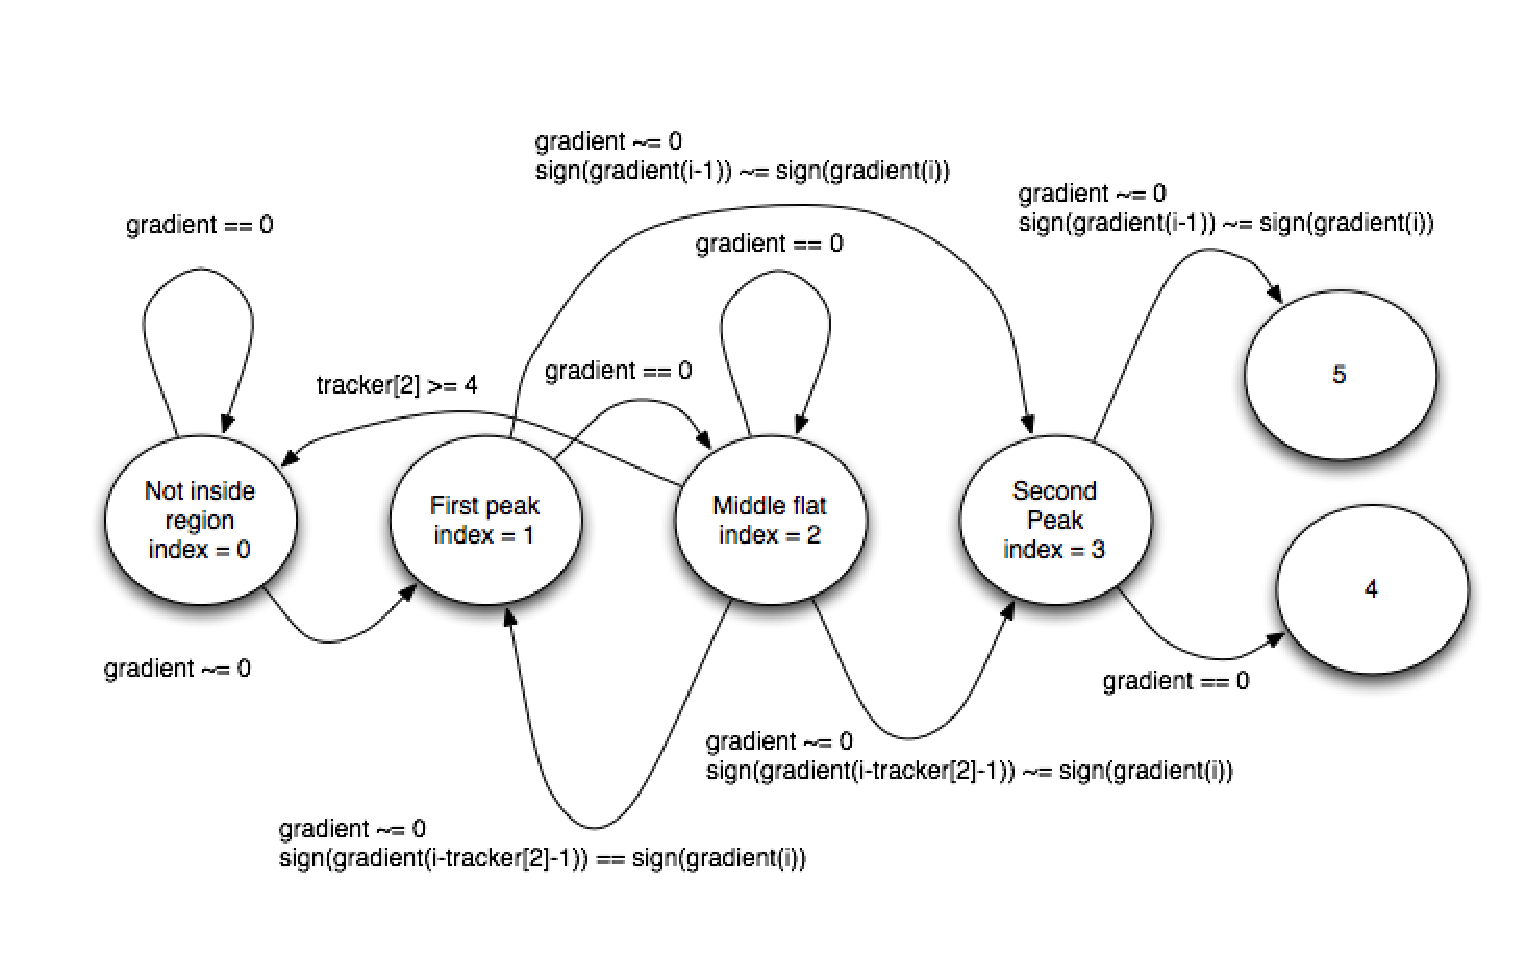
\includegraphics[width=5in]{data_extraction/images/MRI/histogram_state_machine.eps}}}
  \end{minipage}
  \hfill
  \caption{gradient_histogram_state_machine}
  \label{fig:histogram_state_machine}
\end{figure}

\begin{figure}[htb]
  \begin{minipage}[b]{2.5in}
    \centering
    \centerline{\mbox{
\includegraphics[width=2.5in]{data_extraction/images/MRI/1_raw.eps}}}
    \centerline{\emph{(a)}}
  \end{minipage}
  \begin{minipage}[b]{2.5in}
    \centering
    \centerline{\mbox{
\includegraphics[width=2.5in]{data_extraction/images/MRI/2_remove_short_edges.eps}}}
    \centerline{\emph{(b)}}
  \end{minipage}
  \begin{minipage}[b]{2.5in}
    \centering
    \centerline{\mbox{
\includegraphics[width=2.5in]{data_extraction/images/MRI/3_remove_large_bumps.eps}}}
    \centerline{\emph{(c)}}
  \end{minipage}
  \begin{minipage}[b]{2.5in}
    \centering
    \centerline{\mbox{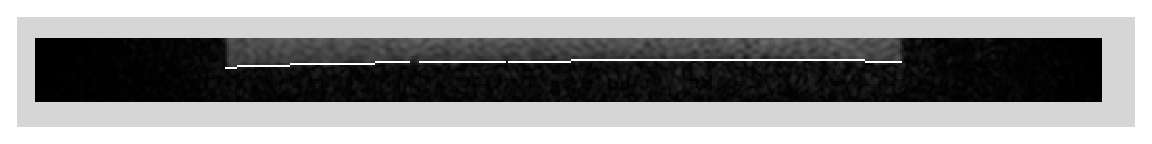
\includegraphics[width=2.5in]{data_extraction/images/MRI/4_removed_peaks.eps}}}
    \centerline{\emph{(d)}}
  \end{minipage}
  \begin{minipage}[b]{2.5in}
    \centering
    \centerline{\mbox{
\includegraphics[width=2.5in]{data_extraction/images/MRI/5_final_edge.eps}}}
    \centerline{\emph{(e)}}
  \end{minipage}
  \caption{MRI surface intermediate edge results: (a) Raw edge (b) after removing short edges (c) after removing large bumps (d) after removing peaks (e) final edge}
  \label{fig:mri_edge_results}
\end{figure}

Using this method, the final surface extracted from MR images for lower tank lower surface is shown in figure
~\ref{fig:surface_result}

\begin{figure}[htb]
  \hfill
  \begin{minipage}[b]{4.5in}
    \centering
    \centerline{\mbox{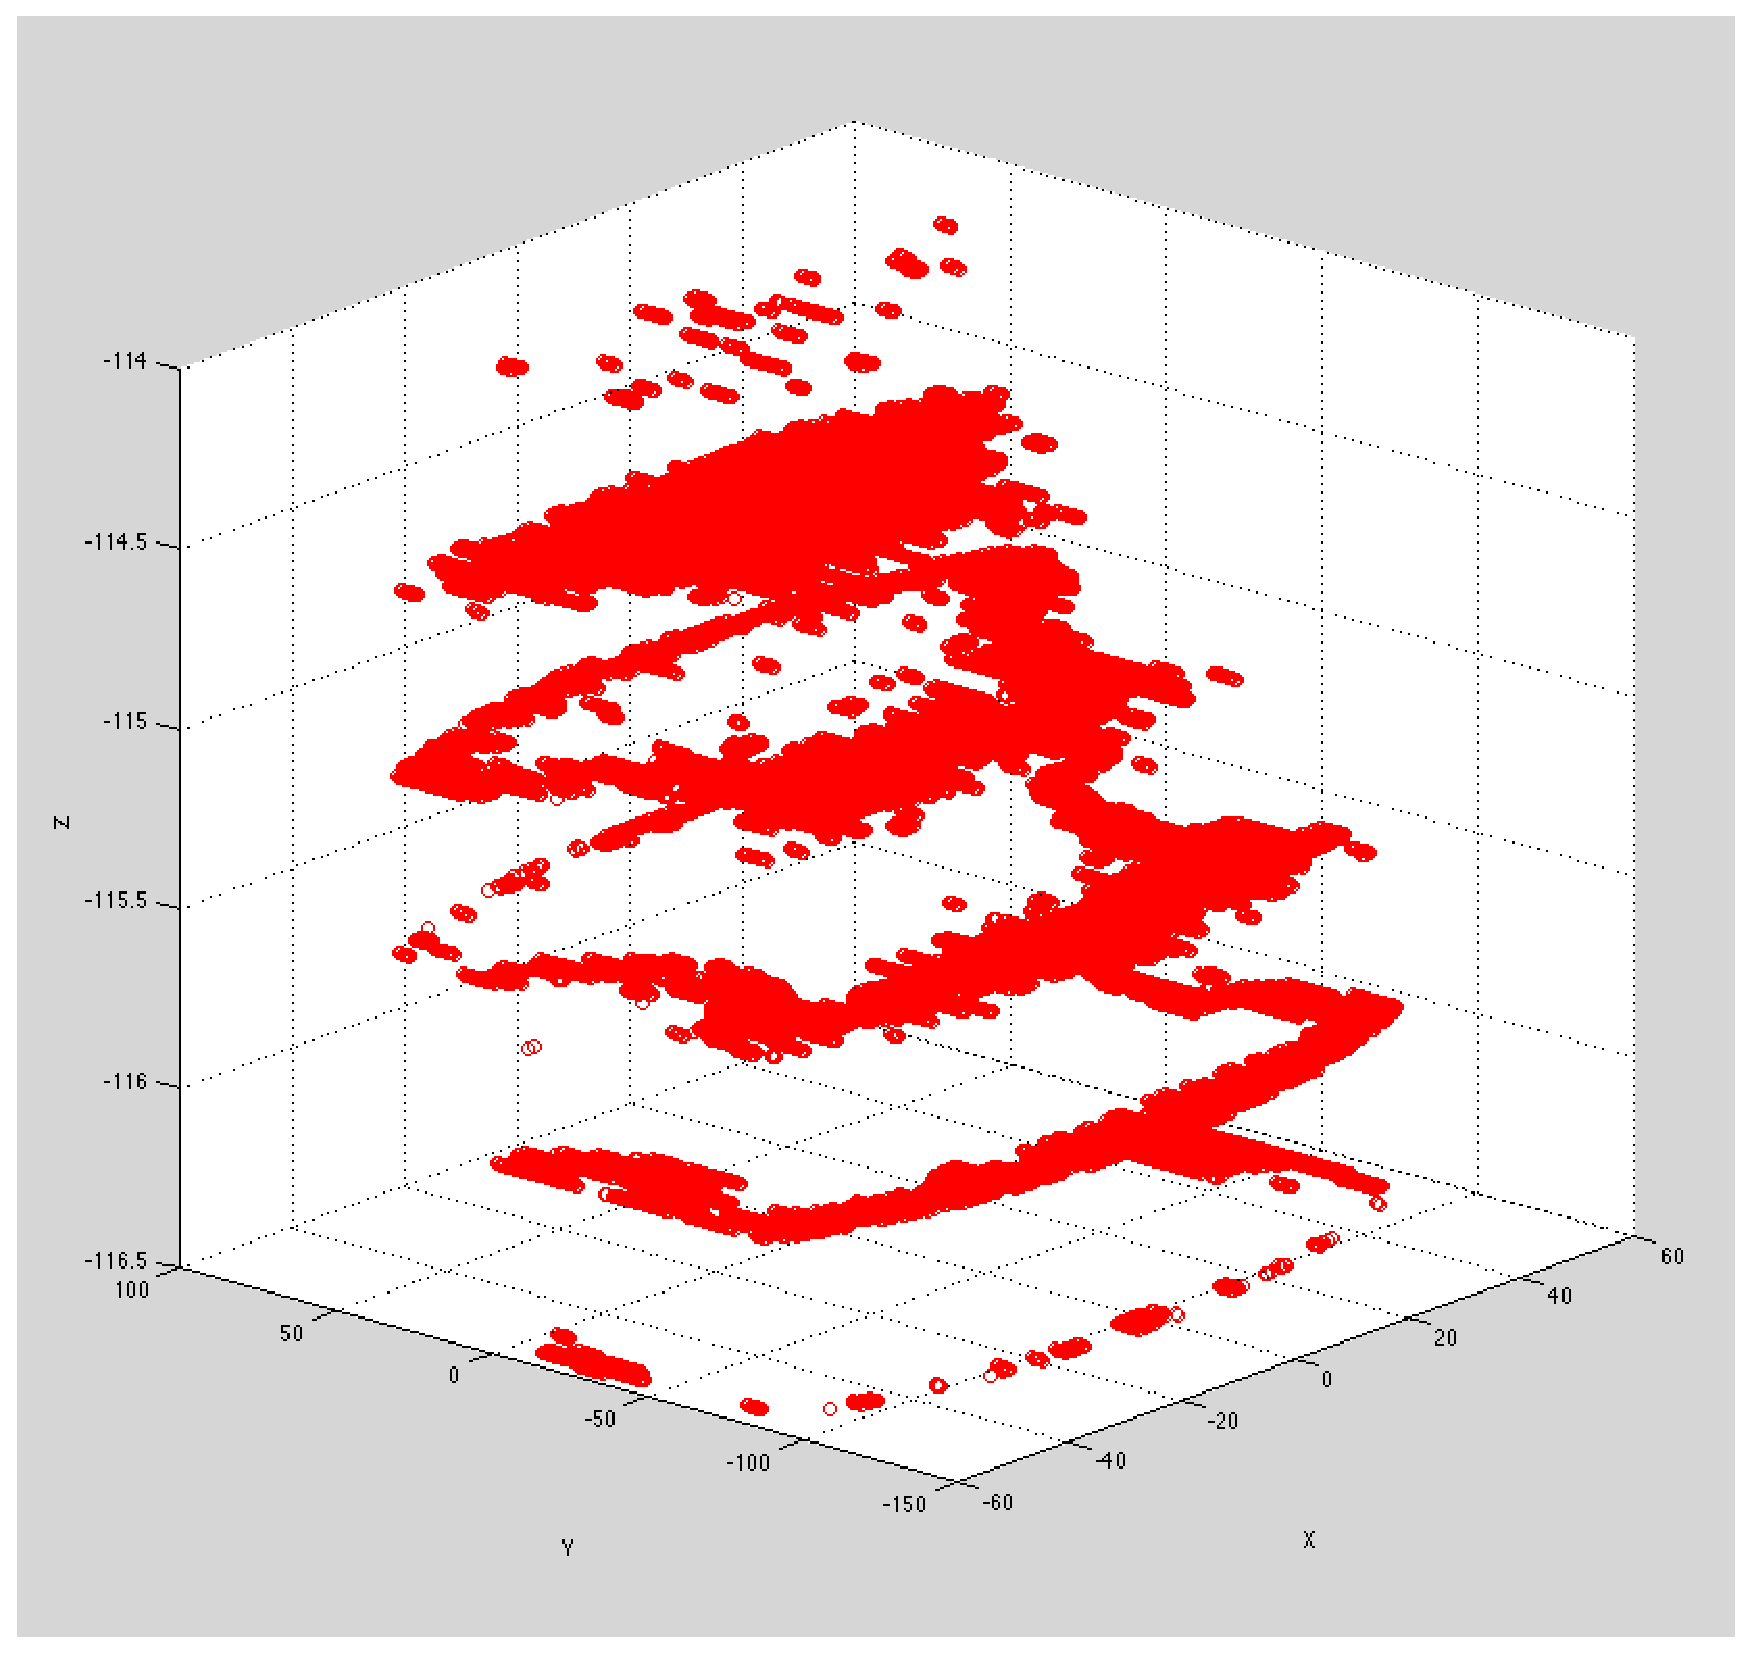
\includegraphics[width=4.5in]{data_extraction/images/MRI/surface4.eps}}}
  \end{minipage}
  \hfill
  \caption{Lower tank lower surface result.}
  \label{fig:surface_result}
\end{figure}



